% Options for packages loaded elsewhere
\PassOptionsToPackage{unicode}{hyperref}
\PassOptionsToPackage{hyphens}{url}
%
\documentclass[
]{article}
\usepackage{amsmath,amssymb}
\usepackage{iftex}
\ifPDFTeX
  \usepackage[T1]{fontenc}
  \usepackage[utf8]{inputenc}
  \usepackage{textcomp} % provide euro and other symbols
\else % if luatex or xetex
  \usepackage{unicode-math} % this also loads fontspec
  \defaultfontfeatures{Scale=MatchLowercase}
  \defaultfontfeatures[\rmfamily]{Ligatures=TeX,Scale=1}
\fi
\usepackage{lmodern}
\ifPDFTeX\else
  % xetex/luatex font selection
\fi
% Use upquote if available, for straight quotes in verbatim environments
\IfFileExists{upquote.sty}{\usepackage{upquote}}{}
\IfFileExists{microtype.sty}{% use microtype if available
  \usepackage[]{microtype}
  \UseMicrotypeSet[protrusion]{basicmath} % disable protrusion for tt fonts
}{}
\makeatletter
\@ifundefined{KOMAClassName}{% if non-KOMA class
  \IfFileExists{parskip.sty}{%
    \usepackage{parskip}
  }{% else
    \setlength{\parindent}{0pt}
    \setlength{\parskip}{6pt plus 2pt minus 1pt}}
}{% if KOMA class
  \KOMAoptions{parskip=half}}
\makeatother
\usepackage{xcolor}
\usepackage[margin=1in]{geometry}
\usepackage{graphicx}
\makeatletter
\def\maxwidth{\ifdim\Gin@nat@width>\linewidth\linewidth\else\Gin@nat@width\fi}
\def\maxheight{\ifdim\Gin@nat@height>\textheight\textheight\else\Gin@nat@height\fi}
\makeatother
% Scale images if necessary, so that they will not overflow the page
% margins by default, and it is still possible to overwrite the defaults
% using explicit options in \includegraphics[width, height, ...]{}
\setkeys{Gin}{width=\maxwidth,height=\maxheight,keepaspectratio}
% Set default figure placement to htbp
\makeatletter
\def\fps@figure{htbp}
\makeatother
\setlength{\emergencystretch}{3em} % prevent overfull lines
\providecommand{\tightlist}{%
  \setlength{\itemsep}{0pt}\setlength{\parskip}{0pt}}
\setcounter{secnumdepth}{-\maxdimen} % remove section numbering
\usepackage{physics}
\ifLuaTeX
  \usepackage{selnolig}  % disable illegal ligatures
\fi
\usepackage{bookmark}
\IfFileExists{xurl.sty}{\usepackage{xurl}}{} % add URL line breaks if available
\urlstyle{same}
\hypersetup{
  pdftitle={The Math},
  hidelinks,
  pdfcreator={LaTeX via pandoc}}

\title{The Math}
\author{}
\date{\vspace{-2.5em}}

\begin{document}
\maketitle

\subsubsection{The Math}\label{the-math}

Consonance perception of a chord with multiple partials is both a wave
and a probabilistic phenomenon.

The probabilistic aspect comes from approximating rational numbers
within a given variance using the Stern-Brocot tree.

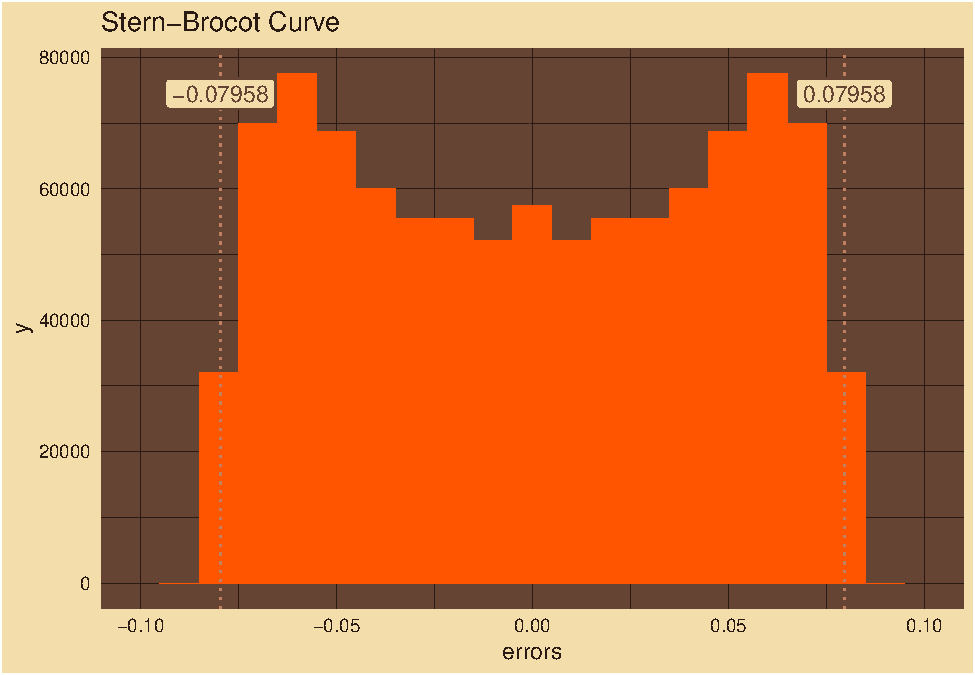
\includegraphics{man/figures/SternBrocotCurve-unnamed-chunk-5-1.pdf}\\
Number of Samples: 1,000,000\\
A peak in a well?\\

\paragraph{Real Traveling Wave}\label{real-traveling-wave}

\[\psi(x,t) = \sin \left( \frac{2\pi x}{\lambda_{0}} - 2 \pi f_{0} t \right)\]

\paragraph{Complex Traveling Wave}\label{complex-traveling-wave}

\[\psi(x,t) = e ^ {-i\left( 2 \pi f_{0} t - \frac{2\pi x}{\lambda_{0}} \right)}\]

\paragraph{State of the Chord}\label{state-of-the-chord}

At time \(t\) the probability for the chord to be in a given state is
given by

\[dP(x) = |\psi(x,t)|^2dx\] It's a probability so the integral must be
one:

\[P(x)=\int|\psi(x,t)|^2dx=1 \]

\subsubsection{Thoughts}\label{thoughts}

\(f(x)\) and \(g(x)\) are both probabilities. The product of their
variance satisfies the uncertainty principle.\\

So what are they in our model?\\

\(f_{0}(f_{i \dots N})\) and \(\lambda_{0}(\lambda_{i \dots N})\) are
probabilities that a set of frequencies or wavelengths will have a
specific fundamental value.\\

\paragraph{Fourier Transform}\label{fourier-transform}

\[\psi({\omega})=\frac{1}{\sqrt{2 \pi}} \int e^{i k {\omega}}\phi(k)dk\]

\[\phi({\vb k})=\frac{1}{\sqrt{2 \pi}} \int e^{-i k \omega}\psi(\omega)d \omega \]
\(\omega\) and \(k\) are vectors.

\paragraph{\texorpdfstring{Now Make \(\psi\) and \(\phi\)
work}{Now Make \textbackslash psi and \textbackslash phi work}}\label{now-make-psi-and-phi-work}

\(\psi\) is temporal, the probability of the fundamental frequency.\\

\(\phi\) is spatial, the probability of the fundamental wavelength.\\

\end{document}
